\documentclass[11pt]{article}
\usepackage[scaled=0.92]{helvet}
\usepackage{geometry}
\geometry{letterpaper,tmargin=1in,bmargin=1in,lmargin=1in,rmargin=1in}
\usepackage[parfill]{parskip} % Activate to begin paragraphs with an empty line rather than an indent %\usepackage{graphicx}
\usepackage{amsmath,amssymb, mathrsfs, dsfont, stackrel}
\usepackage{tabularx}
\usepackage[font=footnotesize,labelfont=bf]{caption}
\usepackage{graphicx}
\usepackage{xcolor}
%\usepackage[linkbordercolor ={1 1 1} ]{hyperref}
%\usepackage[sf]{titlesec}
\usepackage{natbib}
\usepackage{../../Tianpei_Report}
%\usepackage{appendix}
%\usepackage{algorithm}
%\usepackage{algorithmic}

%\renewcommand{\algorithmicrequire}{\textbf{Input:}}
%\renewcommand{\algorithmicensure}{\textbf{Output:}}



\begin{document}
\title{Lecture 6: Instrumental Variables}
\author{ Tianpei Xie}
\date{Sep. 22nd., 2022 }
\maketitle
\tableofcontents
\newpage
\allowdisplaybreaks
\section{What is an Instrument?}
\begin{itemize}
\item How can we identify causal effects when we are in the presence of unobserved confounding? One popular way is to find and use \underline{\emph{\textbf{instrumental
variables}}} \citep{imbens2015causal, peters2017elements, neal2020introduction}. 

\begin{figure}
\begin{minipage}[t]{1\linewidth}
  \centering
  \centerline{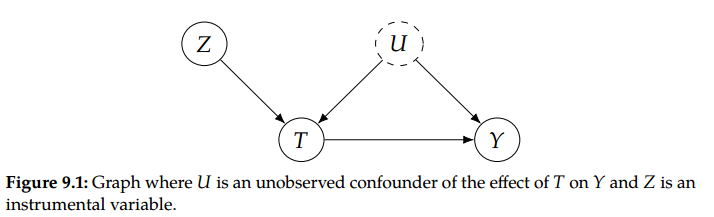
\includegraphics[scale = 0.5]{instrumental_var.png}}
\end{minipage}
\caption{\footnotesize{\textbf{The causal graph for instrumental variable $Z$ \citep{neal2020introduction}}}}
\label{fig: instrumental_var}
\end{figure}

\item \textbf{Instrumental variables (IVs)} is an alternative causal inference technique that does not rely on the ignoreability assumption. That is, it is used when there are \textbf{\emph{unmeasured} confounders}.

\item There are \textbf{three main assumptions} that must be satisfied for a variable to be considered an \emph{\textbf{instrument}}:
\begin{enumerate}
\item \begin{assumption} (\textbf{Relevance})\\
 $Z$ has a causal effect on \textbf{treatment} $T$
\end{assumption}

\item  \begin{assumption} (\textbf{Exclusion Restriction})\\
 $Z$ causal effect on outcome $Y$ is \underline{\textbf{fully mediated}} by treatment $T$
\end{assumption}

\item  \begin{assumption} (\textbf{Instrumental Unconfoundedness})\\
There are \underline{\textbf{no backdoor paths}} from $Z$ to $Y$.
\end{assumption}
\end{enumerate}

\item Intuitively, we interpret the instrumental variable $Z$ as \underline{\textbf{\emph{encouragement}}}, i.e. $Z=1$ would \emph{encourage} the treatment $T=1$ on subject. To guarantee that the \emph{Exclusion Restriction assumption} holds, $Z$ \textbf{should not affect the unobserved confounder} $U$. 

\item This leads to an \emph{\textbf{encouragement design}}. Instead of performing randomized trial on \emph{treatment} $T$, we can \textbf{randomize on the \emph{encouragement}} $Z=1$ vs. $Z=0$. And then an \textbf{\emph{intention-to-treat analysis}} would focus on \emph{the causal effect of \textbf{encouragement}}. 

On the other hand, we would still care about the causal effect of treatment itself, which would be the focus of this chapter.

\item We may consider \emph{treatment \underline{\textbf{assignment}}} as an instrumental variable $Z$ and the \emph{treatment \underline{\textbf{received}}} as the treatment variable $T$. Typically, not everyone assigned treatment will actually receive it (i.e. $Z\neq T$). This lead to \textbf{\emph{randomized trials with \underline{non-compliance}}}. Non-compliance makes the randomized trials look like an observational study. The confounding is based on actual treatment received.

\item For IVs, the \textbf{exclusion restriction} / \textbf{instrumental unconfoundedness} is a strong assumption.
\end{itemize}

\section{Linear Setting}
\subsection{Binary Linear Setting}
\begin{itemize}
\item In this section, we consider the following \emph{noiseless linear causal structure models}
\begin{align}
Y &= \delta\,T + \alpha_{u}\, U \label{eqn: linear_scm}
\end{align} where $U$ is the unobserved confounder. Note that $Z$ does not appear in this equation due to exclusion restriction, since $T$ is determined by $Z$.

\item From \eqref{eqn: linear_scm}, the causal effect of $T$ on $Y$ is defined as $\delta$. To identify $\delta$, we compute
\begin{align*}
&\E{}{Y \,|\, Z = 1} - \E{}{Y \,|\, Z = 0} \\
&= \E{}{\delta\,T + \alpha_{u}\, U \,|\, Z = 1} - \E{}{ \delta\,T + \alpha_{u}\, U \,|\, Z = 0} \\
&= \delta \paren{\E{}{T\,|\, Z = 1} - \E{}{T\,|\, Z = 0}} + \alpha_{u}\paren{\E{}{U\,|\, Z = 1} - \E{}{U\,|\, Z = 0}} \\
& (Z \indep U \text{ by instrumental unconfoundedness}) \\
&= \delta \paren{\E{}{T\,|\, Z = 1} - \E{}{T\,|\, Z = 0}} + \alpha_{u}\paren{\E{}{U} - \E{}{U}} \\
&= \delta \paren{\E{}{T\,|\, Z = 1} - \E{}{T\,|\, Z = 0}}
\end{align*} 

\item \begin{proposition}
The causal effect of $T$ on $Y$ is identified by 
\begin{align}
\delta &= \frac{\E{}{Y \,|\, Z = 1} - \E{}{Y \,|\, Z = 0}}{\E{}{T\,|\, Z = 1} - \E{}{T\,|\, Z = 0}}. \label{eqn: wald_est}
\end{align}
The statistical quantity on the right is called \underline{\textbf{Wald estimand}}.
\end{proposition} 

\item The \emph{\textbf{Wald estimator}} is
\begin{align}
\hat{\delta} &= \frac{\sum_{i: z_i = 1}y_i - \sum_{i: z_i = 0}y_i }{\sum_{i: z_i = 1}t_i - \sum_{i: z_i = 0}t_i} \label{eqn: wald_stats}
\end{align}

\item An alternative explanation for \eqref{eqn: wald_est} is from \emph{causal graphical model} in Figure \ref{fig: instrumental_var}. For linear SCM, the causal association from $T$ to $Y$ is computed by the \emph{\textbf{product of the coefficients}} along the directed path from $T$ to $Y$. Due to the existance of unmeasured confounder $U$, the causal association is not directly measureable. Rather, we can measure total association, and unblocked backdoor paths also contribute to total association, which is why $\E{}{Y\,|\,T=1} - \E{}{Y\,|\,T=0} \neq \delta$. Because there are no backdoor paths from the instrument $Z$ to $Y$, we can trivially identify the effect of $Z$ on $Y$ as $\E{}{Y \,|\, Z = 1} - \E{}{Y \,|\, Z = 0} = \alpha_{z}\delta$. Similarly, we can identify the effect of the instrument on $\E{}{T\,|\, Z = 1} - \E{}{T\,|\, Z = 0} = \alpha_z$. Then, we can divide the effect of $Z$ on $Y$ by the effect of the $Z$ on $T$ to identify $\delta= \frac{ \alpha_{z}\delta}{\alpha_z}$.
\end{itemize}

\subsection{Continuous Linear Setting}
\begin{itemize}
\item We can generalize the setting to continuous $Z$ and $T$, rather than binary. 
\item The Wald estimand for \textbf{continous} $Z$ and $T$ is 
\begin{proposition}
\begin{align}
\delta &= \frac{\text{Cov}(Y\,Z)}{\text{Cov}(T\,Z)}. \label{eqn: wald_est_cont}
\end{align} where $\text{Cov}(A\,B)$ is the cross-covariance between $A$ and $B$.
\end{proposition}
\begin{proof}
\begin{align*}
\text{Cov}(Y\,Z) &= \E{}{Y\,Z} - \E{}{Y}\,\E{}{Z} \\
&= \E{}{\paren{\delta\,T + \alpha_{u}\, U} \,Z} - \E{}{\delta\,T + \alpha_{u}\, U}\,\E{}{Z} \\
&= \delta\,\paren{\E{}{T\,Z} - \E{}{T}\E{}{Z}}+ \alpha_u\,\paren{\E{}{U\,Z} - \E{}{U}\E{}{Z}}\\
& (Z \indep U \text{ by instrumental unconfoundedness}) \\
&= \delta\,\paren{\E{}{T\,Z} - \E{}{T}\E{}{Z}}+ \alpha_u\,\paren{\E{}{U}\E{}{Z} - \E{}{U}\E{}{Z}}\\
&= \delta\,\paren{\E{}{T\,Z} - \E{}{T}\E{}{Z}} = \text{Cov}(T\,Z) \qed
\end{align*}
\end{proof}

\item The \emph{\textbf{Wald estimator}} for continous $Z$ and $T$ is
\begin{align}
\hat{\delta} &= \frac{\widehat{\text{Cov}}(Y\,Z) }{\widehat{\text{Cov}}(T\,Z) } \label{eqn: wald_stats_cont}
\end{align}

\begin{figure}
\begin{minipage}[t]{1\linewidth}
  \centering
  \centerline{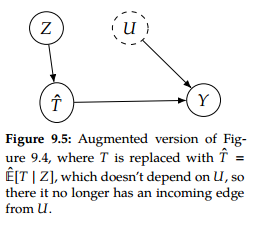
\includegraphics[scale = 0.6]{two_stage_ls.png}}
\end{minipage}
\caption{\footnotesize{\textbf{The two-stage least square process. At first stage, $\widehat{T} = \E{}{T|\,|\,Z}$ replaces $T$, which does not depend on $U$ \citep{neal2020introduction}}}}
\label{fig: two_stage_ls}
\end{figure}



\item An \emph{equivalent estimator} to \eqref{eqn: wald_stats_cont} is \underline{\emph{\textbf{two-stage least square estimator}}}. The two stages are: 
\begin{enumerate}
\item \textbf{Linearly regress} $T$ on $Z$ to estimate $\E{}{T\,|\,Z}$ This gives us the projection $\widehat{T}$ of $T$ onto $Z$; 

At this stage, $T$ is replaced by $\widehat{T}= \E{}{T\,|\,Z}$ which does not depend on $U$. Because $\widehat{T}$ isn't a function of  $U$, we can think of removing the $U \rightarrow \widehat{T}$ edge in this graph. See Figure \ref{fig: two_stage_ls}. 

\item \textbf{Linearly regress} $Y$ on $\widehat{T}$ to estimate $\mathds{E}\,[\,Y\,|\,\widehat{T}\,]$. Obtain our estimate $\hat{\delta}$
as the fitted coefficient in front of $\widehat{T}$.

Because there are no backdoor paths from $\widehat{T}$ to $Y$, we can get that association is causation in stage two, where we simply regress $Y$ on $\widehat{T}$ to estimate the causal effect.
\end{enumerate}
\end{itemize}

\section{Nonparametric Identification of Local ATE}
The problem with approaches above is that we made explicit assumption on the \emph{\textbf{parameteric form}} of causal effect, i.e. the \emph{\textbf{linearity}} assumption. For example, this assumption requires \textit{\textbf{homogeneity}} (that the \emph{treatment effect is the same for every unit}). There are other variants that encode the homogeneity assumption. Ideally, we’d be able to use instrumental variables for identification without making any parametric assumptions such as linearity or homogeneity. 
\subsection{New Potential Notation with Instruments}
\begin{itemize}
\item Define the \underline{\emph{\textbf{potential treatment value}}} $T(1) := T(Z=1) = T^{do(Z=1)}$ and $T(0) := T(Z=0) = T^{do(Z=0)}$ as the treatment we would take if we were to get instrument value $Z=1$ and $Z=0$, respectively.

\item We can define the \textbf{average causal effect of treatment \emph{assignment} on treatment \emph{received}} as
\begin{align}
\E{}{T(1) - T(0)} = \E{}{T^{do(Z=1)}} - \E{}{T^{do(Z=0)}} \label{eqn: causal_effect_treat_assign_to_treat_received}
\end{align}

This is \textbf{the propotion treated} if \emph{\textbf{everyone}} has been assigned to receive the treatment, \textbf{\emph{minus}} the propotion treated if \emph{\textbf{no one}} has been assigned to receive the treatment. If \textbf{perfectly compliance}, this quantity is equal to $1$.

\item We also consider the \textbf{average causal effect of treatment \emph{assignment} on \emph{\textbf{outcome}}}
\begin{align}
\E{}{Y(Z=1) - Y(Z=0)} = \E{}{Y^{do(Z=1)}} - \E{}{Y^{do(Z=0)}} \label{eqn: causal_effect_treat_assign_to_outcome}
\end{align} 
This is the \textbf{average values of outcome} if \emph{\textbf{everyone}} has been assigned to receive the treatment, \textbf{\emph{minus}} the average values of outcome if \emph{\textbf{no one}} has been assigned to receive the treatment. This is also called the \underline{\textbf{\emph{intention-to-treat effect (ITT)}}}. If perfectly compliance, this quantity is equal to the average causal effect (ATE).

\item Due to \emph{\textbf{instrumental unconfoundedness}} and consistency, we can estimate $\E{}{T(1)}= \E{}{T\,|\, Z=1}$ and $\E{}{T(0)}= \E{}{T\,|\, Z=0}$. 
Similarly, we can estimate $\E{}{Y(Z=1)} = \E{}{Y\,|\, Z=1}$ and $\E{}{Y(Z=0)} = \E{}{Y\,|\, Z=0}$.
\end{itemize}

\subsection{Principal Stratification}
\begin{itemize}
\item \begin{definition} (\emph{\textbf{Principal Strata}})  \citep{imbens2015causal, neal2020introduction}
\begin{enumerate}
\item \underline{\textbf{\emph{Compliers}}} - always take the treatment that they are \emph{encouraged} to take. Namely, $T(1) = 1$ and $T(0) = 0$. This is the targeted sub-population.
\item \textbf{\emph{Always-takers}} - always take the treatment, \textbf{regardless} of encouragement. Namely, $T(1) = 1$ and $T(0) = 1$.
\item \textbf{\emph{Never-takers}} - never take the treatment, \textbf{regardless} of encouragement. Namely, $T(1) = 0$ and $T(0) = 0$.
\item \textbf{\emph{Defiers}} - always take the \textbf{opposite treatment} of the treatment that they are \emph{encouraged} to take. Namely, $T(1) = 0$ and $T(0) = 1$.
\end{enumerate}
\end{definition}

\begin{figure}
\begin{minipage}[t]{0.5\linewidth}
  \centering
  \centerline{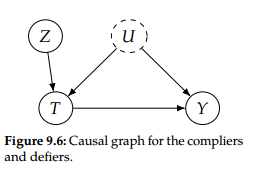
\includegraphics[scale = 0.6]{complier_denier.png}}
  \vspace{-5pt}
  \centerline{(a)}
\end{minipage}
\begin{minipage}[t]{0.5\linewidth}
  \centering
  \centerline{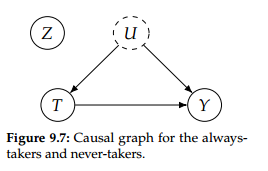
\includegraphics[scale = 0.6]{always_never_takers.png}}
  \vspace{-5pt}
  \centerline{(b)}
\end{minipage}
\caption{\footnotesize{\textbf{The causal graph for (a) complier and defier; (b) always-taker and never taker }}}
\label{fig: principal_strata}
\end{figure}


\item The principal strata is a partition of subjects into four sub-populations. 
\begin{itemize}
\item Clearly, the encouragement will not work for \textbf{Never-takers}. We will \emph{\textbf{not} learn \textbf{anything} on causal effect} of treatment from people in this subpopluation, $P(T=1|\mb{x}) = 0$.
\item For \textbf{Compliers}, they receive treatments when encouraged to, and do not otherwise.  The treatment received in this subpopulation is \emph{\textbf{randomized}}.

\item For \textbf{Defiers},  their treatment received is  also \emph{\textbf{randomized}} but in the \emph{opposite} way. Usually we would image them not existed since normally the group who are not assigned to the treatment has no access to it.

\item For \textbf{Always-takers}, there is \textbf{no information on causal effect} from this subpopulation either since no variations in the treatment received $P(T=0|\mb{x}) = 0$.
\end{itemize} 

\item Given some \textbf{observed} value of $Z$ and $T$, \textbf{we \underline{can’t actually identify} which stratum we’re in}, since we cannot observe the treatment received under the counterfactual treatment assignment. There are four combinations of the binary variables $Z$ and $T$; for each of these combinations, we’ll note that \emph{more than one stratum} is \emph{\textbf{compatible}} with the observed combinations of values.
\begin{enumerate}
\item Given $Z=1$, $T=1$, the compatible strata: \textbf{\emph{compliers}} or \emph{\textbf{always-takers}};
\item Given $Z=1$, $T=0$, the compatible strata: \textbf{\emph{defiers}} or \textbf{\emph{never-takers}};
\item Given $Z=0$, $T=1$, the compatible strata: \textbf{\emph{defiers}} or \emph{\textbf{always-takers}};
\item Given $Z=0$, $T=0$, the compatible strata: \textbf{\emph{compliers}} or \emph{\textbf{never-takers}}.
\end{enumerate}
\end{itemize}

\subsection{Local ATE}
\begin{itemize}
\item A main motivation for using instrument variables is that there exists unobserved confounders. In this situation, the covariate adjustment does not work since we cannot marginalize over \emph{\textbf{all}} confounders.  This means that \textbf{we cannot identify the average treatment effect for the entire population}. 

\item IV methods focus on the identification of \underline{\emph{\textbf{local average treatment effect (LATE)}}}. It is also known as \emph{\textbf{complier average treatment effect (CATE)}}.

\item \begin{definition}\emph{\textbf{(Local Average Treatment Effect (LATE) / Complier Average Causal Effect (CACE))}} \citep{imbens2015causal, neal2020introduction}
\begin{align}
\E{}{Y(T=1) - Y(T=0) \,|\, T(Z=1)=1, \, T(Z=0)=0} = \E{}{Y(1) - Y(0) \,|\, \text{compliers }} \label{eqn: late}
\end{align} It is the average treatment effect conditioned on the \underline{\emph{\textbf{complier sub-populations}}}.
\end{definition}

This is a \emph{causal quantity} since it \textbf{\emph{contrasts counterfactuals}} in a \emph{\textbf{common}} sub-populations. Note that this quantity make no inference on other populations due to no interference assumption.

\item Given observed $Z$ and $T$, the \textbf{challenge} is that we cannot identify the complier directly.

\item To identify the LATE, although we will need to introduce a new assumption.
\begin{assumption} (\textbf{Monotonicity})
\begin{align}
\forall i, \quad  T_i(Z=1) \ge T_i(Z=0) \label{eqn: monotonicity}
\end{align} This is equivalent to say that \underline{\textbf{there is no defier}}. That is, if we are encouraged to take the treatment ($Z = 1$), we are either more likely or equally likely to take the treatment than we would be if we were encouraged to not take the treatment ($Z = 0$).
\end{assumption}

\item Under monotonicity assumption, 
\begin{enumerate}
\item Given $Z=1$, $T=1$, the compatible strata: \textbf{\emph{compliers}} or \emph{\textbf{always-takers}};
\item Given \underline{$Z=1$, $T=0$}, the compatible strata: \underline{\textbf{\emph{never-takers}}};
\item Given \underline{$Z=0$, $T=1$}, the compatible strata: \underline{\emph{\textbf{always-takers}}};
\item Given $Z=0$, $T=0$, the compatible strata: \textbf{\emph{compliers}} or \emph{\textbf{never-takers}}.
\end{enumerate}

\item Under monotonicity assumption,  we can derive the \emph{nonparametric identification} result for the LATE estimand:
\begin{theorem} ({\textbf{LATE Nonparametric Identification}}) \citep{neal2020introduction}\\
Given that $Z$ is an instrument, $Z$ and $T$ are binary variables, and that monotonicity holds, the following is true:
\begin{align}
\E{}{Y(1) - Y(0) \,|\, T(1)=1, \, T(0)=0} &= \frac{\E{}{Y\,|\, Z=1} - \E{}{Y\,|\, Z=0}}{\E{}{T\,|\, Z=1} - \E{}{T\,|\, Z=0}}\label{eqn: late_estimate}
\end{align}
\end{theorem}
\begin{proof}
We’ll start with the causal effect of $Z$ on $Y$ and decompose it into weighted stratum-specific causal effects using the law of total probability:
\begin{align*}
&\E{}{Y^{do(Z=1)} - Y^{do(Z=0)}} \\
&= \sum_{i\in \set{0,1}, j\in \set{0,1}}\E{}{Y^{do(Z=1)} - Y^{do(Z=0)}\,\big|\,T^{do(Z=1)}=i, \, T^{do(Z=0)}=j}P(T^{do(Z=1)}=i, \, T^{do(Z=0)}=j) 
\end{align*}
Note that by monotonicity assumption, $P(T^{do(Z=1)}=0, \, T^{do(Z=0)}=1) = 0$. Morover, the causal effect of always-takers and never-takers are zero. $\E{}{Y|Z, \text{always-takers}} =\E{}{Y|\text{always-takers}}$ and $\E{}{Y|Z, \text{never-takers}} =\E{}{Y|\text{never-takers}}$.  So the LATE is only on complier subset
\begin{align}
&\E{}{Y^{do(Z=1)} - Y^{do(Z=0)}} \nonumber\\
&= \E{}{Y^{do(Z=1)} - Y^{do(Z=0)}\,\big|\,T^{do(Z=1)}=1, \, T^{do(Z=0)}=0}P(T^{do(Z=1)}=1, \, T^{do(Z=0)}=0) \nonumber\\
\Rightarrow  &\quad  \E{}{Y^{do(Z=1)} - Y^{do(Z=0)}\,\big|\,T^{do(Z=1)}=1, \, T^{do(Z=0)}=0} \nonumber\\ 
&= \frac{\E{}{Y^{do(Z=1)} - Y^{do(Z=0)}}}{P(T^{do(Z=1)}=1, \, T^{do(Z=0)}=0)} \label{eqn: ate_z_y}
\end{align}

For complier, the treatment received will equal to treatment assigned so $Y^{do(Z=i)} = Y^{do(T=i)}$ for $i\in \set{0,1}$. So we can rewrite the LHS of \eqref{eqn: ate_z_y} as
\begin{align}
\E{}{Y(1) - Y(0)\,\big|\,T(1)=1, \, T(0)=0} &= \frac{\E{}{Y(Z=1)} - \E{}{Y(Z=0)}}{P(T(1)=1, \, T(0)=0)} \label{eqn: late_1}\\
&  \text{ by instrumental unconfoundedness} \nonumber\\
&=  \frac{\E{}{Y\,|\, Z=1} - \E{}{Y\,|\, Z=0}}{P(T(1)=1, \, T(0)=0)}  \label{eqn: late_2}
\end{align}

Note that we cannot identify the complier from observation alone, but we can identify the never-takers ($T=0 \,|\, Z=1$) and always-takers $(T=1\,|\,Z=0)$ due to monotonicity assumption.  So 
\begin{align}
P(T(1)=1, \, T(0)=0) &= 1 - P(T(1)=0, \, T(0)=0)  - P(T(1)=1, \, T(0)=1) \nonumber\\
&= 1 - P(T=0  \,|\, Z= 1) - P(T=1 \,|\, Z= 0)    \nonumber\\
&= P(T=1  \,|\, Z= 1) - P(T=1 \,|\, Z= 0) \label{eqn: complier_prob} \\
&= P\paren{\text{always-taker \emph{OR} complier}} -  P\paren{\text{always-taker}} > 0\nonumber
\end{align}
So substituting \eqref{eqn: complier_prob}   
\begin{align}
\E{}{Y(1) - Y(0)\,\big|\,T(1)=1, \, T(0)=0} &=  \frac{\E{}{Y\,|\, Z=1} - \E{}{Y\,|\, Z=0}}{P(T=1  \,|\, Z= 1) - P(T=1 \,|\, Z= 0)}  \label{eqn: late_3} \\
&= \frac{\E{}{Y\,|\, Z=1} - \E{}{Y\,|\, Z=0}}{\E{}{T\,|\, Z=1} - \E{}{T\,|\, Z=0}} \nonumber
\end{align} The last equality holds since $T$ is binary variable. \qed


\end{proof}

\item Same as result under linear setting, the LATE estimand is identified by \textbf{Wald estimand}:
\begin{align*}
\text{LATE} = \delta &= \frac{\E{}{Y\,|\, Z=1} - \E{}{Y\,|\, Z=0}}{\E{}{T\,|\, Z=1} - \E{}{T\,|\, Z=0}} = \frac{\text{Average Causal Effect (ITT) }(Z \rightarrow Y)}{\text{Average Causal Effect }(Z \rightarrow T)}.
\end{align*} Different from \eqref{eqn: wald_est}, the Wald estimand is used to compute the \emph{local} ATE. Because there are \emph{no backdoor paths} from the instrument $Z$ to $Y$. Both the \emph{\textbf{average causal effect of treatment assignment on outcome (ITT)}} and the \emph{\textbf{average treatment effect of treatment assignment on treatment received}} are \underline{\textbf{identifiable}}. 

\item If perfect complier, $\text{LATE} = \text{ITT}$; otherwise $\text{LATE} \ge  \text{ITT}$.

 ITT is an \underline{\textbf{\emph{under-estimate}}} of the LATE since there are some people who were assigned to the treatment but did not take it.
\end{itemize}

\section{Instrumental variables in observational studies}
\begin{itemize}
\item The instrumental variables can be thought of a randomizer in the natural experiment. 

\item The key challenge is to think of a variable that affects the treatment but does not affect the outcome \emph{directly}. Note that only assumptions that affect the treatment can be checked with observations. 

\item The validity of exclusion restriction and instrumental unconfoundedness largely depends on the domain expertise.

\item For example, the \emph{\textbf{calandar time}} can be used as an IV, e.g. the treatment probability change over time and $Z$ can be early time period vs. late time period. In order to make sure exclusion restriction, the other treatment practices and patient behaviors should not change during two different time periods. 

\item Also, the \emph{\textbf{distance}} to a specialty care center is used as an IV for health outcomes.

\item The health care provider preference, i.e. the treatment prescribed to previous patients, can be used as an IV.

\item \emph{\textbf{Mendelian randomization}}:  some genetic variant is associated with some behavior (e.g. alcohol use), but is assumed to not be associated with the outcome.

\item In these observational settings, we can still think about \emph{\textbf{compliance}}, i.e compliance with encouragement. 

\item In practice, it is always helpful to perform \textbf{sensitivity analysis} on the exclusion restriction assumption ("what would change if $Z$ \emph{directly affect} $Y$ by a given amount $\rho$?") and the monotonicity assumption ("what would change if the proportion of defier is $\pi$?").
\end{itemize}
\subsection{Weak instruments}
\begin{itemize}
\item The strength of an IV is how well it \textbf{predicts} the treatment received.
\begin{itemize}
\item A \emph{\textbf{strong} instrument} is highly predictive of the treatment received. That is, the encouragement will greatly increase the probability of treatment;
\item A \emph{\textbf{weak} instrument} is weakly predictive of the treatment received. That is, the encouragement will barely increase the probability of treatment.
\end{itemize}

\item We can measure the \underline{\emph{\textbf{strength of instrumental variable}}} using the \textbf{\emph{probability of compliers}} 
\begin{align}
\E{}{T\,|\,Z=1} - \E{}{T\,|\,Z=0} \label{eqn: strength_iv}
\end{align}

\item A weak instrument can cause problems.  Suppose only $1\%$ of population are compliers, the amount of samples is $1\%\,n$ for a total of $n$ samples. The \textbf{limited sample size} would cause \textbf{high variance} for estimators. The causal effect estimator is unstable. 

\item If IV is weak, an IV analysis may not be the best option. There are researches to \textit{strengthen} the IV (using \emph{\textbf{near/far matching}} for example).
\end{itemize}

\newpage
\bibliographystyle{plainnat}
\bibliography{book_reference.bib}
\end{document}